%* 
%* ------------------------------------------------------------------
%* ResistorManual.tex - Resistor Manual
%* Created by Robert Heller on Wed Mar 19 14:53:24 2008
%* ------------------------------------------------------------------
%* Modification History: $Log$
%* Modification History: Revision 1.1  2002/07/28 14:03:50  heller
%* Modification History: Add it copyright notice headers
%* Modification History:
%* ------------------------------------------------------------------
%* Contents:
%* ------------------------------------------------------------------
%*  
%*     Model RR System, Version 2
%*     Copyright (C) 1994,1995,2002-2005  Robert Heller D/B/A Deepwoods Software
%* 			51 Locke Hill Road
%* 			Wendell, MA 01379-9728
%* 
%*     This program is free software; you can redistribute it and/or modify
%*     it under the terms of the GNU General Public License as published by
%*     the Free Software Foundation; either version 2 of the License, or
%*     (at your option) any later version.
%* 
%*     This program is distributed in the hope that it will be useful,
%*     but WITHOUT ANY WARRANTY; without even the implied warranty of
%*     MERCHANTABILITY or FITNESS FOR A PARTICULAR PURPOSE.  See the
%*     GNU General Public License for more details.
%* 
%*     You should have received a copy of the GNU General Public License
%*     along with this program; if not, write to the Free Software
%*     Foundation, Inc., 675 Mass Ave, Cambridge, MA 02139, USA.
%* 
%*  
%* 

\chapter{Resistor Program Reference}
\label{chpt:rest:Reference}
\typeout{$Id$}

The Resistor Calculator program aids in calculating dropping resistors
for LEDs and low-voltage lamps commonly used on model railroads.  It
implements Ohm's Law\index{Ohm's Law}, shown in
Equations~\ref{eq:rest:OhmsLaw} and~\ref{eq:rest:VDrop} to perform the
calculation and then finds the nearest stock value and also displays
the color bands for typical carbon resistors.

\begin{eqnarray}
R_{drop} &=& \frac{V_{drop}}{I} \label{eq:rest:OhmsLaw} \\
V_{drop} &=& V_{supply} - V_{load} \label{eq:rest:VDrop}
\end{eqnarray}

The calculator takes three input values, the supply voltage
($V_{supply}$), the voltage across the load ($V_{load}$) (LED or lamp)
and the load current ($I$) the LED or lamp operates at.  These values
are entered along with the units they are in. Then the calculate button
is pushed and the results are displayed.  The results can also be saved
to a text file, which can be printed or otherwise refered to later.

\begin{figure}[hbpt]
\begin{centering}
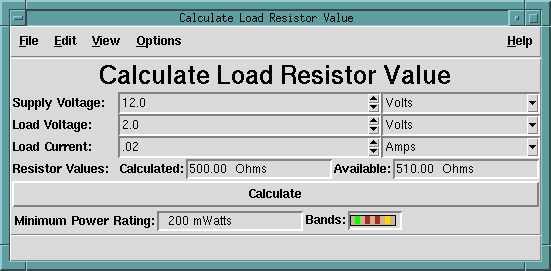
\includegraphics[width=5in]{RestMain.png}
\caption{The main GUI screen of the Resistor Calculator program}
\label{fig:rest:Main}
\end{centering}
\end{figure}
The main GUI screen of the Resistor Calculator program is shown in
Figure~\ref{fig:rest:Main}.  

